% do not change these two lines (this is a hard requirement
% there is one exception: you might replace oneside by twoside in case you deliver 
% the printed version in the accordant format
\documentclass[11pt,titlepage,oneside,openany]{book}
\usepackage{times}

%personally added
\usepackage{color}

\usepackage{graphicx}
\usepackage{latexsym}
\usepackage{amsmath}
\usepackage{amssymb}


\usepackage{ntheorem}

% \usepackage{paralist}
\usepackage{tabularx}

% this packaes are useful for nice algorithms
\usepackage{algorithm}
\usepackage{algorithmic}

% well, when your work is concerned with definitions, proposition and so on, we suggest this
% feel free to add Corrolary, Theorem or whatever you need
\newtheorem{definition}{Definition}
\newtheorem{proposition}{Proposition}


% its always useful to have some shortcuts (some are specific for algorithms
% if you do not like your formating you can change it here (instead of scanning through the whole text)
\renewcommand{\algorithmiccomment}[1]{\ensuremath{\rhd} \textit{#1}}
\def\MYCALL#1#2{{\small\textsc{#1}}(\textup{#2})}
\def\MYSET#1{\scshape{#1}}
\def\MYAND{\textbf{ and }}
\def\MYOR{\textbf{ or }}
\def\MYNOT{\textbf{ not }}
\def\MYTHROW{\textbf{ throw }}
\def\MYBREAK{\textbf{break }}
\def\MYEXCEPT#1{\scshape{#1}}
\def\MYTO{\textbf{ to }}
\def\MYNIL{\textsc{Nil}}
\def\MYUNKNOWN{ unknown }
% simple stuff (not all of this is used in this examples thesis
\def\INT{{\mathcal I}} % interpretation
\def\ONT{{\mathcal O}} % ontology
\def\SEM{{\mathcal S}} % alignment semantic
\def\ALI{{\mathcal A}} % alignment
\def\USE{{\mathcal U}} % set of unsatisfiable entities
\def\CON{{\mathcal C}} % conflict set
\def\DIA{\Delta} % diagnosis
% mups and mips
\def\MUP{{\mathcal M}} % ontology
\def\MIP{{\mathcal M}} % ontology
% distributed and local entities
\newcommand{\cc}[2]{\mathit{#1}\hspace{-1pt} \# \hspace{-1pt} \mathit{#2}}
\newcommand{\cx}[1]{\mathit{#1}}
% complex stuff
\def\MER#1#2#3#4{#1 \cup_{#3}^{#2} #4} % merged ontology
\def\MUPALL#1#2#3#4#5{\textit{MUPS}_{#1}\left(#2, #3, #4, #5\right)} % the set of all mups for some concept
\def\MIPALL#1#2{\textit{MIPS}_{#1}\left(#2\right)} % the set of all mips


% custom stuff
\usepackage[hidelinks]{hyperref}


\begin{document}

\pagenumbering{roman}
% lets go for the title page, something like this should be okay
\begin{titlepage}
	\vspace*{2cm}
  \begin{center}
   {\huge Mining the Success for Movies \\}
   \vspace{2cm} 
   {\Large Student Project Data Mining HWS17\\
   Team 6\\}
   \vspace{2cm}
   {\Large Presented by \\}
   \vspace{0.5cm}
    {Steffen Jung \\
    Adrian Kochsiek \\
    Martin Koller \\
    Marvin Messenzehl \\
    Daniel Szymkowiak \\
   }
   \vspace{1cm} 
   { Submitted to the\\
    Data and Web Science Group\\
    Prof.\ Dr.\ Heiko Paulheim\\
    University of Mannheim\\} \vspace{2cm}
   {October - December 2017}
  \end{center}
\end{titlepage} 

% no lets make some add some table of contents
\tableofcontents
\newpage

%\listofalgorithms

%\listoffigures

%\listoftables

% evntuelly you might add something like this
% \listtheorems{definition}
% \listtheorems{proposition}

\newpage


% okay, start new numbering ... here is where it really starts
\pagenumbering{arabic}

%%%%%%%%%%%%%%%%%%%%%%%%%%%%%%%%%%%%%%%%

% INPUTS
%\chapter{Application Area and Goals}\label{cha:area_goals}
\begingroup
\renewcommand{\cleardoublepage}{}
\renewcommand{\clearpage}{}
\chapter{Application Area and Goals}\label{chap:area_goals}
\endgroup


This paper represents a documentation of the data mining project \textit{"Mining the Success for Movies"}\footnote{Information in this paper refers to the (sample) dataset and python scripts handed in for a classification problem. The repository can be found at \hyperref{https://github.com/yOoMarvin/movie-mining}{external}{github}{on GitHub under: https://github.com/yOoMarvin/movie-mining}}. The structure of this paper follows the classical data mining process: The data selection and preprocessing are covered in chapter \ref{cha:data_selection} and the data mining with an evaluation of results and a prospect are covered in chapter \ref{cha:data_mining}.

%Chapter \ref{cha:area_goals} provides an overview of the problem the project is based on and is complemented by the goals and objectives of this project. Afterwards, chapter \ref{cha:data_selection} deals with the structure and size of the data. Here, a closer look will be taken at the dataset at hand. %Questions that had to be answered were for example which information was provided in the original dataset or which problems were identified concerning for instance outliers or missing values. 
%Upon that, chapter \ref{cha:preprocessing} explains which preprocessing steps had to be taken in order to cleanse the dataset to prepare it for the data mining step and model learning introduced in chapter \ref{cha:data_mining}. Here, the used data mining techniques are described regarding algorithms and parameters that were used to learn an expedient models in respect of the goals set in Chapter \ref{cha:area_goals}. Additionally, gained insights of the problem at hand are presented and a critical reflection is delineated how the model could be improved further in order to provide even more precise results.

\paragraph{Problem Statement}
Before new movies are being produced, every stakeholder is interested in the monetary success of the intended movie. In order to predict the success, costly methods are being applied, such as market investigations or analyses. The benefit of Data Mining to the analysis of large datasets can also be transferred to the stated problem of predicting a movie's success. %In order to learn and apply the model, various pieces of information are taken into account. Just a few are budget, revenues, runtime, genre and information on the release. Information on the dataset and on all preprocessing methods which were applied will be provided in chapter \ref{cha:data_selection}.

\paragraph{Goals}
The goal of this project is to learn a model which will predict how successful a not yet released movie will be. This is done by using common data mining techniques in the Python programming language. Several packages were used for different tasks. For example, the packages \textit{pandas} and \textit{numpy} were used for working with dataframes and numerical values. For creating graphics and plots, the chosen package was \textit{matplotlib}. In addition to that, parts of the  Python machine learning library \textit{scikit learn} were used for building classification models and evaluating them. As the main objective the question \textit{"Based on revenue, will the movie be popular or will it be a flop?"} shall be answered for all possible combinations of information on a new movie as precisely as possible.
%In order to be as precise as possible, not only different algorithms are being tested, but also parameter tuning is being applied with different performance measures \footnote{Further information on applied techniques and evaluation methods is provided in chapter \ref{cha:data_mining}}.








 
\chapter{Data Selection and Preprocessing}
\label{cha:data_selection}

\section{Structure of data and data exploration}
\label{sec:data_exploration}
The selected dataset onto which a classification model shall be learned is provided by Kaggle\footnote{2017 Kaggle Inc}. It is named \textit{The Movies Dataset}\footnote{Link to the dataset: \hyperref[https://www.kaggle.com/rounakbanik/the-movies-dataset]{https://www.kaggle.com/rounakbanik/the-movies-dataset}} and contains metadata of approximately 45,000 movies in its raw format. It is provided and updated by Rounak Banik. The complete dataset consists of several files in \textit{csv}-format containing data about movie casts, metadata and external scores. The main file used during preprocessing is named \textit{movies-metadata.csv}. This \textit{csv}-file contains 24 columns, which can be seen in the graphic below. In addition to that, information from the file \textit{credits.csv} is also extracted. It is described in section \ref{cha:preprocessing}.
\begin{figure}[ht]
	\centering
		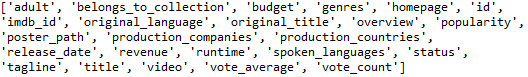
\includegraphics[width=\textwidth]{images/Raw_dataset_headers.png}
	\caption{Columns of the file \textit{movies-metadata.csv}}
\end{figure}

%Due to the multitude of attributes, it is essential to extract the relevant values for the implementation of a well-functioning classifier. Many values have no effect on the financial success of a movie and can therefore be ignored. This includes, for example, the columns...

The structure of the individual columns is very different. In addition to boolean values, strings and numeric float values (e.g \textit{budget} or \textit{runtime}), many attributes contain longer texts (e.g \textit{overview}), arrays or even a list of JSON objects (e.g. \textit{production\_countries}). The different formats must be taken into account in the preprocessing and need to be processed and extracted individually.
%\\\\
%\section{Basic data exploration}

The overall quality of the dataset varies significantly. This can be due to the fact that it is maintained by a community and is not provided by a larger organization or company. Therefore, a demanding quality assurance process is difficult to realize. It is an important quality aspect of a dataset that it contains values for the majority of its records. The examined dataset has a high amount of records containing missing values. This is the case especially for elder movies (before 1960), which contain only few information. Critical for this project is the availability of the attribute values \textit{revenue} and \textit{budget}, which are used to determine the financial success of the movie. Here around 34,000 records are containing zero or missing values in either the \textit{revenue} or the \textit{budget} column.

In addition to that, there is no indication about the currencies of numerical financial attributes. Also, values are inconsistent in respect to scaling. For example a movie having an actual revenue of \$ 312MM and a budget of \$ 240MM is given with a \textit{revenue} value of \textit{240,000,000} as a float number whereas the \textit{budget} value contains the float number \textit{312}. Another source of inconsistency is discovered after randomly cross-checking the values contained in the dataset with available box office numbers online. These checks indicate that different market assumptions (e.g. US market only vs. worldwide) were taken into account for the values contained in the dataset. For the successful outcome of this project it is crucial to keep those aspects in mind for later preprocessing steps, otherwise the results will be distorted.

Speaking of those issues it is also worth mentioning that the chosen dataset contains movie metadata from the past 60 years. With respect to today's economics a lot of things changed in movie production and consumption. Aspects that have influenced movie economics are for example price structures, inflation and globalization. Naturally, also consumer behavior changed drastically. Therefore, it was decided to introduce a new attribute to the dataset called \textit{productivity}. 
\begin{wraptable}{l}{0.55\textwidth}
	\begin{tabular}{| l | l |}
	\hline
	Average budget & \$ 31,662,585 \\ \hline
	Average revenue & \$ 92,059,210 \\ \hline
	Average productivity & 2.8 \\ \hline
	Most common genres & Drama, Comedy,\\ & Thriller \\ \hline
	Average runtime & 94 min. \\ \hline
	\end{tabular}
	\caption{Basic insights from the dataset}
	\label{tbl:insights}
\end{wraptable} 
The \textit{productivity} describes the ratio of \textit{revenue} and \textit{budget} of a movie and expresses its success in this project. A \textit{productivity} of $1.0$ implies that the budget to produce the movie was covered and anything above $1.0$ is assumed as profit.
%\\
In order to get a better understanding of the data and its relations, table \ref{tbl:insights} presents some average numbers of crucial columns and the most common genres.

\section{Preprocessing Data}
\label{cha:preprocessing}

In total, two datasets were used to create features for testing the different classifiers:
\textit{movies\_metadata.csv} and \textit{credits.csv}. The dataset \textit{movies\_metadata.csv} contains 45,463 rows and 23 columns excluding the id-column. The dataset \textit{credits.csv} contains 45,463 rows and 2 columns excluding the id-column.

\paragraph{Vertical scaling.}
Both dimensions for the dataset \textit{movies\_metadata.csv} were processed. As section \ref{sec:merge_create} explains, the revenue and budget played a major role for the data mining task. Therefore all datasets without information on each column had to be dropped out, which was a major part of the dataset. Also duplicates were identified using the ID and discarded. 
 
After this, the dataset shrunk to roughly 4000 rows. To retain some numbers and still use datasets which had only missing out revenue or budget two approaches were implemented: A parser for the IMDB database\footnote{
\hyperref{http://www.imdb.com/}{external_sources}{ref:IMDB}{The IMDB database: http://www.imdb.com/}} API and for the The Numbers\footnote{\hyperref{http://www.the-numbers.com/research-analysis}{external_sources}{ref:numbers}{the numbers website: http://www.the-numbers.com/research-analysis}} API was programmed and run. With these approaches it was possible to gain the real values of budget and revenue for the dataset. By mining two of the most reliable movie-datasources out in the web, it was also possible to determine rows, which used foreign currency values in their revenue or only revenue based on the local market (e.g. only in the US).

\paragraph{Horizontal scaling.}
Based on the assumptions that budget and revenue were crucial numbers, also other features have been selected for the modeling. A special focus has been placed on the following datacolumns: the release year, the genre, the production country as well as the production company, the spoken languages, the runtime and the fact whether a movie belongs to a collection or not. Due to high encoding effort for these features, further columns are not taken into account during this project. Figure \ref{img:mm_columns} gives an overview on which information was retained.

The reason why information, which could have been potentially interesting, had to be dropped, was mainly for time reasons. Preprocessing took about 70\% of the timeperiod\footnote{Mainly due to the fact that heaps of problems arose from the dataset, which can be read in chapter \ref{cha:data_selection}.} of the whole project. Thus, the team was able to focus on preprocessing of mentioned columns. Still, chapter \ref{cha:data_selection} provides a prospect, which steps were possible, if a larger time frame was dedicated to this project.

After dropping out information, eleven columns remained. Combined with the two columns from the \textit{credits.csv} dataset, thirteen columns were used as a basis to create features for finding the best performing classifiers.

In order to transform the data into a suitable representation for forecasting a movie's success, preprocessing was mandatory. For each column zero or more preprocessing steps from the following list were performed:
\\ \\
\fbox{\begin{minipage}{\textwidth}
\textit{Merging of columns, discretization (binning) of features, extracting information out of columns, one hot encoding normalizing.}
\end{minipage}}
\\ \\
The following sections explain the preprocessing in detail. Figure \ref{img:features} shows precisely, which operations were executed on each column and how the data types changed.


\paragraph{Merging and creating columns.}
\label{sec:merge_create}



When a new movie is planned, the finances are one of the most important concerns. Where the budget can be circumscribed upfront, revenue is nearly impossible to guess. As a result, the prediction of a model should consider the revenue as a key factor for it's monetary success. To only predict the revenue (using multiple bins or binary binning, like e.g. "will the revenue of a new movie be higher or lower than \$500,000?") would not have worked out due to multiple reasons: Both the revenue and budget of a movie in earlier years, like e.g. the 1950's, was
\begin{wrapfigure}{l}{0.7\textwidth}
	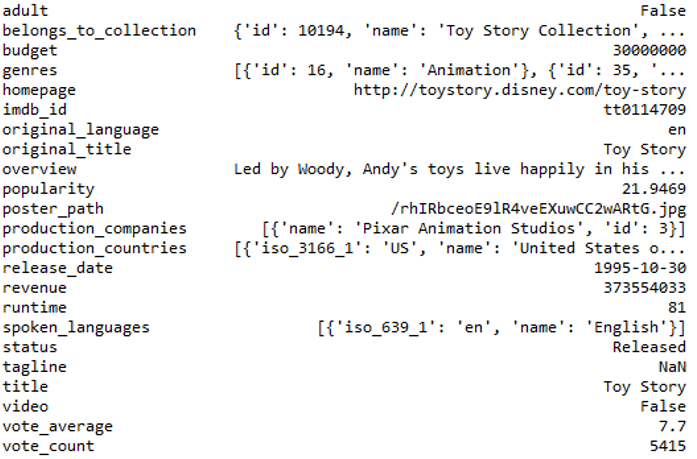
\includegraphics[width=0.7\textwidth]{images/3_metadata_columns.png}
	\caption{Remained columns of \textit{movies\_metadata.csv} are highlighted in yellow}
	\label{img:mm_columns}
\end{wrapfigure}
\FloatBarrier
 considerably less than today, so total numbers are not comparable. Additionally, inflation plays a role in comparing financial numbers of elder movies to newer ones. Furthermore, the dataset contained different currencies like dollars, euros or indian rupees without indicating which currency was provided per dataset.
 
As described in chapter \ref{sec:data_exploration}, a new column had to be introduced, namely the productivity. It is a quotient, computed by dividing revenue through budget. If the productivity is higher than one, the movie derives profit, if the productivity is less than one, the movie derives a loss. That way, above mentioned issues can be avoided. The column revenue was dropped afterwards.

Considering the release date of a movie, the assumption was made that the demand for movies is higher in quarter four of the year (time of winter and christmas). This was confirmed by checking the numbers\footnote{Check for details on revenues in video-selling: \hyperref{https://de.statista.com/statistik/daten/studie/182319/umfrage/umsatzentwicklung-im-video-kaufmarkt-quartalszahlen/}{link}{Statista revenue movies}{https://de.statista.com/statistik/daten/studie/182319/umfrage/umsatzentwicklung-im-video-kaufmarkt-quartalszahlen/}}. Hence, a new column of numeric type with quarter one to four was created. The previous column release date was converted to release year only as a numeric format.

\paragraph{Discretization.}
During this preprocessing step, the created column productivity was binned two ways: Once multi-binned into four different bins having bins between 0.0 to 0.99 (label "\textit{unproductive}"), 1.0 to 1.99 (label "\textit{smallProductivity}"), 2.0 to 4.99 (label "\textit{goodProductivity}") and 5.0 to infinity (label "\textit{highProductivity}"), and once binary-binned into two bins having 0.0 to 0.9 (label "\textit{no}") and 1.0 (label "\textit{yes}") to infinity. For each bin a new column was added, the former productivity column was dropped.

\paragraph{Extracting information.}
As stated in chapter \ref{cha:data_selection} some information, including the production companies, actors and crew members is provided as a JSON Object inside a column of the dataset. 

The first approach, taken into account contained parsing of the JSON data. However, some columns contained invalid JSON format and therefore made the processing very cumbersome.

However, after a closer analysis of the values inside the column, a new extraction concept could be developed. Given the values of the cast column, actors could be extracted by looking for the regular expressions inside the correlating values. For example actors could be identified by looking for the parameter name, and extracting the value provided by the parameter. The same procedure with slight changes has been applied to the extraction of the production companies, the directors and the countries of production.

After evaluation of the extracted parameters, inconsistent values for the production companies have been discovered. These inconsistent values contain for example: "Twenty Century Fox", "Twenty Century-Fox" and "Twenty Century Fox Production". Without any further preprocessing each of the values would be one hot encoded separately. Therefore a second step of preprocessing has been performed to remove different ways of writing the same company, and therefore providing similar values for one hot encoding.
 
\paragraph{Normalizing, thresholding and one hot encoding.}
Not only the in the previous step extracted information on genre, production country, production company director and actor was one hot encoded using the pandas get\_dummies()\footnote{The \hyperref{https://pandas.pydata.org/pandas-docs/stable/generated/pandas.get_dummies.html}{documentation}{pd.getDumies}{Documentation on pandas get\_dummies() function can be found online}} function, but also the original language. After one-hot-encoding, the dataset consisted of about 49000 columns\footnote{The high number is due to the high number of different actors, directors, production companies and production countries.}.

In order to reduce the amount of columns and to filter out unnecessary data a threshold had been applied. For example actors, directors and companies, which are not frequently participating in the movie-production-scene have been eliminated using a filter. Thus it can be assured that only actors et. al are taken into account which participated in a reasonable amount of movies, and therefore have an impact on the classifier.

In order to create equal meaning among the different numeric values in the data set some of the columns, including runtime, budget and year, are normalized using MinMax scaling.

\begin{figure}[htbp]
	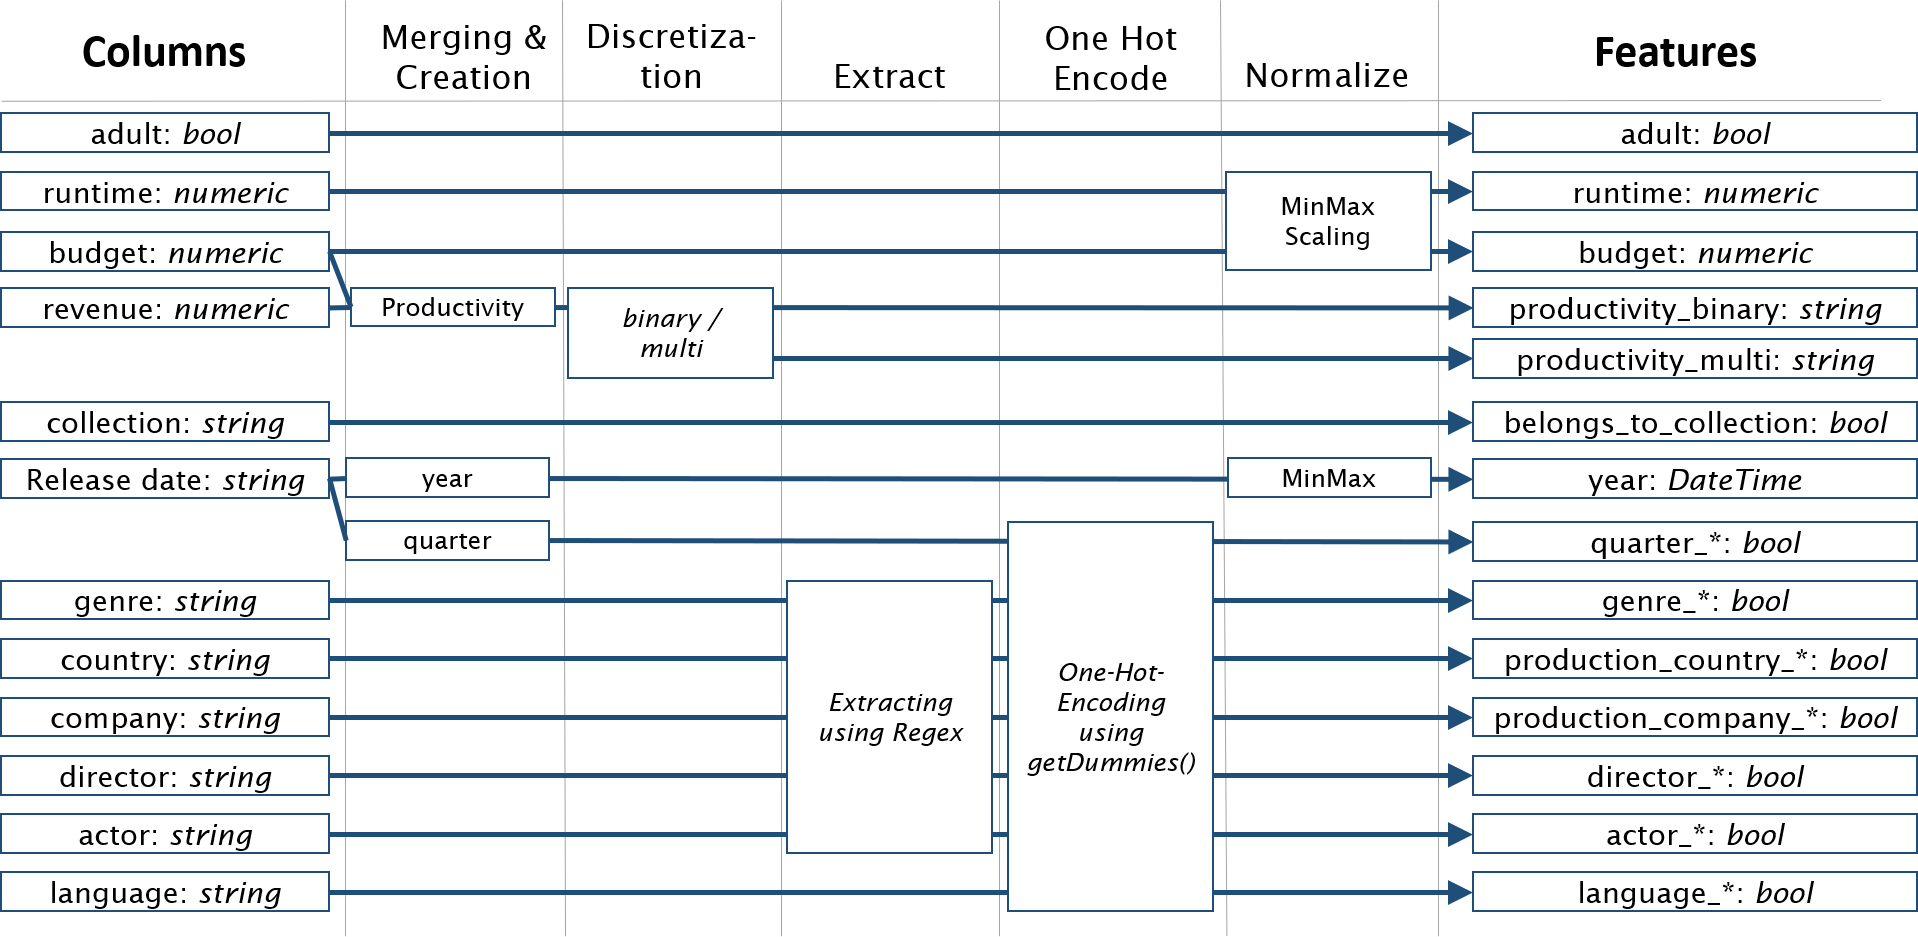
\includegraphics[width=\textwidth]{images/3_features.png}
	\caption{Features created during preprocessing}
	\label{img:features}
\end{figure}
\FloatBarrier

%\begin{itemize}
%	\item Transform data into a representation that is suitable for the chosen data mining methods
%	\begin{itemize}
%		\item number of dimensions
%		\item scales of attributes (nominal, ordinal, numeric)
%		\item amount of data (determines hardware requirements)
%	\end{itemize}
%	\item Methods
%	\begin{itemize}
%		\item Aggregation, sampling
%		\item Dimensionality reduction / feature subset selection
%		\item Attribute transformation / text to term vector
%		\item Discretization and binarization
%	\end{itemize}
%	\item Good data preparation is key to producing valid and reliable models
%	\item Data preparation estimated to take 70-80\% of the time and effort of a data mining project!
%\end{itemize}

%\section{A list of problems we encountered}
%\begin{enumerate}
%	\item \textbf{list further problems we had and solved!}
%	\item Prod. Comp.: Same prod. company named differently -> using Regex to solve (Steffen)
%	\item dataset: 5 datasets have duplicates
%\end{enumerate}

\chapter{Data Mining}
\label{cha:data_mining}

After preprocessing the data, the next step is to build a classifier to predict the success of a movie. To find the best classifier a set of different algorithms is evaluated:
K-nearest neighbor (kNN), 
na\"{i}ve bayes, 
support vector classifier (SVC), 
neural net, 
decision tree and 
random forest.

The first goal of the analysis was to predict the success in four different classes. Since an analysis in that detail with the given data set is very unprecise, a binary classifier was created.
For all of the named algorithms an individual feature selection is applied to get the best results. The important features are selected by a greedy feature wrapper. This feature wrapper starts with the full set of features and drops features as long as the result improves. The results are checked with a stratified 10-fold cross-validation. Additionally to the selection of features, thresholding for features like the number of actors and number of production companies can be applied. For example actors, directors and companies, which are not frequently participating in the movie-production-scene can be eliminated. Thus it can be assured that only columns are taken into account which are contained in a reasonable amount of movies, and therefore have an impact on the classifier. \\
In the next step some hyperparameter tuning is needed to improve the classifiers. To find the best parameter setting, a grid search in combination with a stratified 10-fold cross-validation, scoring the highest F1-score (macro), is applied to the classifiers.
The achieved F1-scores of the three best binary classifier are listed in table \ref{tab:binary_classifier}. 

Previous tests using the micro F1-score have shown, that even though promising results could be scored, the classifiers only learned guessing the majority in this setting. Therefore the F1-score had been changed to macro,
%At first the classifiers are scoring the micro F1-score. Even though the result looks promising at the beginning, the classifier are mostly guessing the majority class in this setting. For that reason every classifier is scoring on the macro F1-score.
 since the dataset for the binary classifier is unbalanced with a ratio of 75\% "successful" and 25\% "unsuccessful". Therefore another test to improve the classifiers is to balance the train set.
%That for the stratified cross-validation is used to balance the train set.
That for the stratified cross-validation is extended with an optional argument to balance the train set by down- or upsampling.
%For further improvement
The train set can be downbalanced by shrinking the majority class to the size of the minority class. However, test series showed that downsampled training sets result in lower performance scores of the classifiers. It is assumed that the reason is the already small dataset.
%But since the dataset is already small after the preprocessing, the downsampling worsens the classifiers.
To not shrink the dataset any further upsampling can be applied to increase the minority class of the train set to the size of the majority class. However, also this sampling technique showed a decrease in performance.

In the following section the the two best performing classifiers - kNN and SVC - are examined in more detail.
\begin{figure}[h]
	\center
	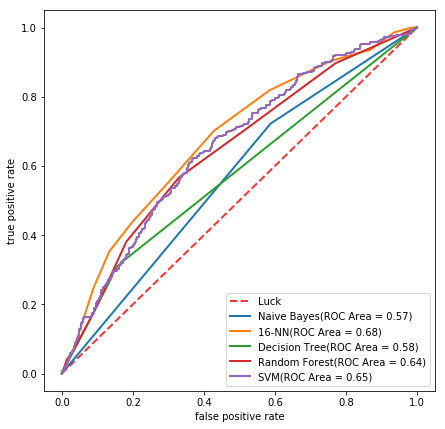
\includegraphics[width=0.7\textwidth]{images/roc.png}
	\caption{Macro average ROC Curves for all classifiers}
	\label{img:roc}
\end{figure}


% Please add the following required packages to your document preamble:
% \usepackage{booktabs}
%% \usepackage{graphicx}
%\begin{table}[]
%\centering
%\resizebox{\textwidth}{!}{%
%\begin{tabular}{@{}lllll@{}}
% & k-NN & SVM & SVM &  \\
%thresholds & actor: 8 company:3 director:3 & actor: 8 company: 3 director: 3 & no threshold &  \\
%columns dropped & 'actor\_', 'quarter\_', 'genre\_', 'country\_', 'runtime', 'adult' & 'quarter\_', 'adult', 'actor\_', 'director\_' & 'country\_', 'genre\_', 'runtime', 'adult', 'actor\_', 'director\_' &  \\
%hyperparameter & \begin{tabular}[c]{@{}l@{}}'algorithm': 'auto', 'metric': 'euclidean', 'n\_neighbors': 16,\\   'p': 2, 'weights': 'uniform'\end{tabular} & class\_weight': 'balanced', 'multi\_class': 'ovr' & no parameters &  \\
%precision &  &  &  &  \\
%recall &  &  &  &  \\
%F1 (macro) & 0,6141 & 0,6069 & 0,5777 & 
%\end{tabular}%
%}
%\caption{My caption}
%\label{my-label}
%\end{table}

\begin{center}
\begin{table}
	\begin{tabular}{ | p{2,5cm} | p{2,5cm} | p{2.5cm} | p{3cm}|}
    \hline
   Thresholds & k-NN & SVM & NB\\ \hline
    Columns dropped & actor\_, quarter\_, genre\_, country\_, runtime, adult & quarter\_, adult, actor\_, director\_ & country\_, genre\_, runtime, adult, actor\_, director\_  \\ \hline
    hyperparameter & algorithm= auto, metric= euclidean, neighbors= 16, p= 2, weights= uniform & class\_weight= balanced, 'multi\_class= ovr & no parameters  \\ \hline
    Precison&  &  &  \\ \hline
	recall &  &  &   \\ \hline
	F1(macro) & 0,6141 & 0,6069 & 0,5777 \\ \hline
    
    \end{tabular}
    \caption{Results overview} 
   \label{tab:values}
\end{table}
\end{center}
\section {Classifiers}
\paragraph{K nearest neighbor}
After the preprocessing the dataset is highly dimensional with more than 50,000 columns. Even though kNN does not work very well on a high dimensional dataset, the algorithm is the best performing one with a good feature selection. After dropping all the actors, country, genre and quarter information and limiting the director and the companies to the ones that took part at at least three movies of the data set, the classifier scores an F1 score of 61.4\%. The algorithm is comparing the labels of the 16 nearest neighbors calculated with the euclidean distance. Both down- and upsampling worsens the classifier. 

\paragraph{Support vector classifier}
As the kNN the support vector classifier works best after dropping a lot of features. Without any information to the actors, country, quarter, genre and age limitation and limiting the companies and directors to the ones that took part at at least three movies, the classifier scores an F1 score of 60.7\%. For the best result the algorithm works with a linear kernel and a balanced class weight. Both down- and upsampling worsens the classifier.

%\paragraph{Decision Tree}
%One way to deal with the issue of an unbalanced data set is to use a tree-structured classifier, since the hierarchical structure allows them to learn signals from both classes.
%To find the best parameter setting for the decision tree the grid-search tests the parameters split criterion, max depth, minimum samples to split and the class weight in a ten fold cross-validation. After dropping the "quarter", "runtime" and "adult" columns, the classifier scores without any sampling, no class weight, an entropy split criterion and a max depth of 100 an F1 score of 58\%. Both the down- and the upsampling worsens the classifier.

%\paragraph{Random Forest}
%Like the decision tree, random forest builds  a hierarchical structure, which can handle unbalanced data sets better than other algorithms. In addition it corrects the overfitting habit of a decision tree. In the gridsearch hyperparameters like the split-criterion, number of features, the minimum sample to split and whether bootstrap samples are used or not are evaluated. After dropping the actors and the release quarter, the classifier scores a F1 score of 59\%. As with the decision tree neither down- nor upsampling the train set improves the result.
\section{Evaluation and Prospect}
\paragraph{Evaluation}

\label{cha:prospect}

As discovered in the previous paragraphs, some classifiers perform better than others. One reason could be seen in the amount of data in the data set. The final data set of about 3,900 rows can be considered as small. Therefore, as shown in the ROC curves above, decision tree and random forest are not performing the best scores. Usually they rely on large dataset, where they can evaluate data more efficiently. The random forest however, scores an higher accuracy since it takes knowledge from various trees inside the forest.



Other classifiers as for example na\"{i}ve bayes perform not as well as the trees. One possible reason could be that na\"{i}ve bayes assumes that no correlation between the features exist. However, in this specific task movies with more famous actors usually generate a bigger budget. 

Best scores are reached with the kNN and the SVC. The kNN classifier works best with values close to the training example, as it calculates the distance between the features. An object itself is than classified by the majority votes of each neighbor.
SVCs bring best results if there are various training examples with a known distribution. Both are applied best to the given dataset and therefore perform most reliable.







%\begin{itemize}
%	\item very small dataset -> not all algorithms perfom very well
%	\item Example numbers -> some perform better: why? 
%	\item Analysis of values
%\end{itemize}


\chapter{Interpretation / Evaluation}
\label{cha:interpretation_evaluation}
Maybe also prospect?
\begin{itemize}
	\item Output of Data Mining
	\begin{itemize}
		\item Patterns
		\item Models
	\end{itemize}
	\item In the end, we want to derive value from that, e.g.,
	\begin{itemize}
		\item gain knowledge
		\item make better decisions
		\item increase revenue
	\end{itemize}
\end{itemize}
\chapter{Prospect}
Perspective of the project
\label{cha:prospect}
\begin{itemize}
	\item find other data sources for revenue / budget values to expand the data set with additional movies
	\item try other feature selection methods (backward wrapper, filter)
	\item add additional features
	\begin{itemize}
		\item popularity of the actors / crew
		\item add additional crew members (e.g. writer)
		\item extract key phrases from the synopsis of the movie
	\end{itemize}
\end{itemize}

%\input{./content/outline.tex}

%\bibliographystyle{plain}
%\bibliography{literature}




%not needed as stated in dws_vorlage
%\appendix

%\chapter{Program Code / Resources}
%\label{cha:appendix-a}

%The source code, a documentation, some usage examples, and additional test results are available at ...

%They as well as a PDF version of this thesis is also contained on the CD-ROM attached to this thesis.

%\chapter{Further Experimental Results}
%\label{cha:appendix-b}

%In the following further experimental results are ...




\newpage


\pagestyle{empty}


%\section*{Ehrenw\"ortliche Erkl\"arung}
%Ich versichere, dass ich die beiliegende Master-/Bachelorarbeit ohne Hilfe Dritter
%und ohne Benutzung anderer als der angegebenen Quellen und Hilfsmittel
%angefertigt und die den benutzten Quellen w\"ortlich oder inhaltlich
%entnommenen Stellen als solche kenntlich gemacht habe. Diese Arbeit
%hat in gleicher oder \"ahnlicher Form noch keiner Pr\"ufungsbeh\"orde
%vorgelegen. Ich bin mir bewusst, dass eine falsche Er- kl\"arung rechtliche Folgen haben
%wird.
%\\
%\\

%\noindent
%Mannheim, den 31.08.2014 \hspace{4cm} Unterschrift

\end{document}
